\chapter{Literature Review}

\label{ch:Literature Review}

\section{Theoretical Foundation}

\subsection{Orbital Angular Momentum of Light}
\label{ssec:oam of light}

在古典電磁學與現代量子光學中，光子不僅攜帶線性動量，亦具備角動量。光學角動量通常可明確區分為 SAM 與 OAM 兩個部分。SAM 與光波的圓偏振狀態密切相關，主要表現為光場向量的旋轉性質；而 OAM 則取決於光場的空間幾何分佈，特別是與波前的空間相位結構息息相關。
在物理機制上，電磁場的總角動量密度 $\mathbf{J}$ 可以透過坡印廷向量來定義，其數學表達式如公式所示：
\begin{align}
\mathbf{J} = \mathbf{E} \times \mathbf{H}
\end{align}
其中，$\mathbf{E}$ 為電場強度向量，$\mathbf{H}$ 為磁場強度。在標準的近軸近似條件下，假設光束沿著 $z$ 軸傳播，此時電磁場的縱向分量遠小於橫向分量。在此近似架構下，透過空間積分，總角動量 $\mathbf{J}$ 可以嚴格且完備地拆解為SAM $\mathbf{S}$ 與OAM $\mathbf{L}$ 的獨立線性疊加：
\begin{align}
\mathbf{J} = \mathbf{S} + \mathbf{L}
\end{align}
此公式即代表 SAM 與 OAM 完全分離，在傳播過程中不會發生內部的能量交換或動量耦合。

對於具有螺旋波前的光束而言，其電場複數振幅在圓柱坐標系 $(r, \phi, z)$ 下包含一個特定的方位角結構因子 $e^{i\ell\phi}$。根據量子力學詮釋，光束中的每一個光子皆攜帶確定的 OAM 值，其特徵關係式如公式所示：
\begin{align}
L_z = \ell\hbar
\end{align}
在此公式中，$L_z$ 代表沿傳播方向的OAM 分量，$\ell$ 為拓撲荷，其值必須為整數以滿足空間波動方程式的邊界條件，而 $\hbar$ 則為約化普朗克常數。這種由空間相位梯度所引導的物理機制，會在光場中產生圍繞傳播軸線的坡印廷向量螺旋環流，進而形成宏觀上的 OAM。

\subsection{Spin-Orbit Interaction}

然而，當光學系統進入非近軸範疇，上述 SAM 與 OAM 將不再獨立。在強聚焦系統中，光線會以極大的角度向中心匯聚，使得波前發生劇烈彎曲，並在焦點附近形成極具空間不均勻性的橫向電場分佈。此時，其橫向空間梯度 ($\partial E_x/\partial x$ 與 $\partial E_y/\partial y$) 將會大幅增加，為了滿足馬克士威方程式中的高斯定律：
\begin{align}
\nabla \cdot \mathbf{E} = \frac{\partial E_x}{\partial x} + \frac{\partial E_y}{\partial y} + \frac{\partial E_z}{\partial z} = 0
\end{align}
系統必然會產生顯著的縱向電場分量 $E_z$，其振幅大小與橫向分量 $E_x, E_y$ 相當，在數學計算與物理效應上皆不可忽略。這種由幾何邊界與波前結構驅動的場分量耦合轉換，便是引發光學自旋軌道交互作用 (Spin-Orbit Interaction, SOI) 的核心機制。

為了具體量化此物理現象，以攜帶 SAM ($s = \pm 1$) 的圓偏振高斯光束經過高數值孔徑透鏡強聚焦為例。當入射光為左旋圓偏振 (LCP, $s = +1$) 時，其入射電場可表示為：
\begin{align}
\mathbf{E}_{in} = \mathbf{E}_{0} (r,z) (\hat{x} + is\hat{y})e^{ikz}
\end{align}
若將公式轉換至柱座標系，則可展開為：
\begin{align}
\mathbf{E}_{\text{in}} \propto (\hat{x} + is\hat{y}) = (\cos\phi \hat{\rho} - \sin\phi \hat{\phi}) + is(\sin\phi \hat{\rho} + \cos\phi \hat{\phi})
\end{align}
當光線經透鏡聚焦傾斜 $\theta$時，由於方位角分量 ($\hat{\phi}$ 項) 始終與 $z$ 軸垂直，只有徑向分量 ($\hat{\rho}$ 項) 會投影到 $z$ 軸。單獨提取 $\hat{\rho}$ 前面的係數，其幾何投影關係為：
\begin{align}
\text{Projection to } z \propto \cos\phi + is\sin\phi
\end{align}
根據歐拉公式，可以進一步簡化：
\begin{align}
\cos\phi + is\sin\phi = e^{is\phi}
\end{align}
在 Richards-Wolf 高NA聚焦理論中，焦點總電場是透過對透鏡孔徑面上的平面波進行二維角譜積分 (對傾角 $\theta$ 與方位角 $\phi_p$ 積分) 得到。在計算縱向電場分量 $E_z$ 的過程中，對孔徑面方位角 $\phi_p$ 的環向積分步驟如下：
\begin{align}
E_z \propto \int_0^{2\pi} (\cos\phi_p + is\sin\phi_p) e^{ik\rho\cos(\phi_p - \phi)} d\phi_p
\end{align}
透過變數變換，這項積分可以改寫為：
\begin{align}
\int_0^{2\pi} e^{is\phi_p} e^{ik\rho\cos(\phi_p - \phi)} d\phi_p = e^{is\phi} \int_0^{2\pi} e^{is\alpha} e^{ik\rho\cos\alpha} d\alpha
\end{align}
這時，方位角相位 $e^{is\phi}$ 被提到了積分符號外面。而右手邊剩下的積分項，根據貝索函數的積分定義，剛好正比於一階第一類貝索函數 $J_1(k\rho\sin\theta)$ 。

因此，經高 NA 透鏡聚焦後，焦平面 ($z=0$) 附近的縱向電場分量 $E_z(\rho, \phi, z)$ 經由上述座標變換與角譜積分，可嚴格推導為：
\begin{align}
E_{z}= (\rho, \phi, z) = -iAe^{is\phi}I_{1}(\rho,z)
\end{align}
其中，$A$ 為振幅常數。$I_1(\rho, z)$ 為與透鏡聚焦角度 (即數值孔徑 $\text{NA} = n\sin\alpha$) 相關的重疊積分項，其數學定義為：
\begin{align}
I_1(\rho, z) = \int_0^\alpha \cos^{1/2}\theta \sin^2\theta P(\theta) J_1(k\rho\sin\theta) e^{ikz\cos\theta} d\theta
\end{align}
此處 $\theta$ 為聚焦傾角，$\alpha$ 為最大聚焦半角，$P(\theta)$ 為切趾函數，而 $J_1$ 則為一階第一類貝索函數。

從公式中 $E_z$ 的數學形式可以發現，縱向電場分量中自發性地衍生出了項為 $e^{is\phi}$ 的相位因子，這正是拓撲荷為 $\ell = s = + 1$ 的光學渦旋相位。意即，原本純粹由偏振狀態決定的 SAM ($s = + 1$)，在強聚焦的幾何邊界約束下，透過空間梯度的幾何耦合，一部分能量被具體轉換成了帶有螺旋波前的 OAM ($\ell = + 1$)。這個現象闡明了光學自旋軌道交互作用中 SAM 到 OAM 轉換的物理機制。

\subsection{Laguerre–Gaussian Modes}  
\label{sec:lg}

亥姆霍茲方程式奠定了自由空間中單色光束的傳播行為。當光束沿 $z$ 軸前進時，近軸波動方程式控制了其電場振幅在橫截面上的演化：
\begin{align}
\left( \frac{\partial^2}{\partial r^2} + \frac{1}{r}\frac{\partial}{\partial r} + \frac{1}{r^2}\frac{\partial^2}{\partial \phi^2} + 2ik\frac{\partial}{\partial z} \right) u(r,\phi,z) = 0
\end{align}
此方程式為柱座標系下的解析解，代表光束除了常見的高斯分佈外，還存在一整組具有特殊幾何對稱性的拉格耳-高斯（Laguerre-Gaussian, LG）光束。

這類光束最核心的物理特徵，在於其波前不再是傳統的平面或單純的球面，而是隨著傳播軸向呈螺旋狀扭曲的幾何結構。此物理現象源於分離變數法中，方位角分量所引入的空間相位因子 $\exp(i\ell\phi)$。為了滿足波動場在圍繞傳播軸旋轉 $2\pi$ 後必須回到原狀態的單值邊界條件，方位角指數 $\ell$ 被限制為整數 ($\ell = 0, \pm 1, \pm 2, \dots$)，在光學中稱為拓撲荷。當 $\ell \neq 0$ 時，光束在空間中前進一單位波長，其等相位面便會圍繞中心軸旋轉 $\ell$ 個週期，形成宏觀上的螺旋波前。螺旋波前的存在，導致光束中心軸 ($r=0$) 成為一個相位奇點，來自各個方位的波包因相位互不相容而產生完全破壞性干涉。

因此，在完整的 $LG_{p,\ell}$ 三維複振幅模型中：
\begin{align}
u_{p,\ell}(r, \phi, z) = \sqrt{\frac{2p!}{\pi(p+|\ell|)!}} \frac{1}{w(z)} \left( \frac{\sqrt{2}r}{w(z)} \right)^{|\ell|} L_p^{|\ell|}\left( \frac{2r^2}{w^2(z)} \right) e^{ -\frac{r^2}{w^2(z)}} e^{ \frac{ikr^2}{2R(z)}} e^{i\ell\phi} e^{-i(2p+|\ell|+1)\psi(z)}
\end{align}
其中 $\psi(z)$ 為 Gouy 相位，徑向項 $\left(\frac{\sqrt{2}r}{w(z)}\right)^{|\ell|}$ 確保了中心原點處的振幅與強度恆為零。當最基礎的空心螺旋模態 (徑向指數 $p=0$) 在空間中傳播時，其橫截面強度 $I = |u_{0,\ell}|^2$ 的極大值精確落在半徑 $r_{\text{max}} = w(z)\sqrt{\ell/2}$ 的圓環上。這使得 LG 光束在空間中如圓環狀般的中空強度場形，且中空強度半徑會隨著拓撲荷 $|\ell|$ 的增大而呈根號關係擴張。

從微觀動力學的角度來看，將 LG 光束的電磁場代入時間平均坡印廷向量 $\langle\mathbf{S}\rangle = \frac{1}{2}\text{Re}\{\mathbf{E} \times \mathbf{H}^*\}$ 可以發現，在近軸近似下，能量流動的方位角分量 $S_\phi$ 與縱向分量 $S_z$ 的物理關聯：
\begin{align}
\frac{S_\phi}{S_z} = \frac{\ell}{kr}
\end{align}
此關係式表明，電磁能量不再單純沿著 $z$ 軸直線前進，而是圍繞著傳播軸產生了角動量流密度。這意味著 LG 光束中的每個光子，除了自身偏振所決定的 SAM 之外，還額外攜帶了與拓撲荷成正比的 OAM，其量值精確為每個光子 $\ell\hbar$。這種由空間幾何結構所衍生出的 OAM，正是 LG 光束能對微觀粒子產生光學力矩、驅使粒子繞軸旋轉的物理本質。

\subsection{Monolayer Transition Metal Dichalcogenides: Crystal Structure, Band Structure, and Valley Physics}

\subsubsection*{晶體結構與空間反轉對稱性破缺}

單層過渡金屬二硫屬化物 (Transition Metal Dichalcogenides, TMDs) 的化學通式為 MX$_2$，其中 M 為過渡金屬原子 (如 Mo、W)，X 為硫屬原子 (如 S、Se)。在晶體結構上，單層 MX$_2$ 由一層過渡金屬原子夾在兩層硫屬原子之間所構成，形成 X-M-X 三明治結構，過渡金屬原子與六個最近鄰硫屬原子形成三角棱柱配位。

在體材形式下，TMDs 具有空間反轉對稱中心 (屬 $D_{3d}$ 點群)，使布里淵區邊界的 $K$ 與 $K'$ 谷在能量上等價，導致體材 TMDs 為間接能隙半導體。然而，當材料厚度減薄至單原子層極限時，由於層間配位的消失，晶格的空間反轉對稱性遭到打破，點群由 $D_{3d}$ 降低為 $D_{3h}$。這一對稱性破缺具有深遠的物理意義：$K$ 與 $K'$ 谷成為布里淵區中兩個不等價的高對稱點，材料由間接能隙轉變為直接能隙半導體 \cite{mak2010atomically, splendiani2010emerging}，並為谷自由度的存在與谷選擇光學躍遷奠定了根本的結構前提。

\begin{figure}[H] 
\centering 
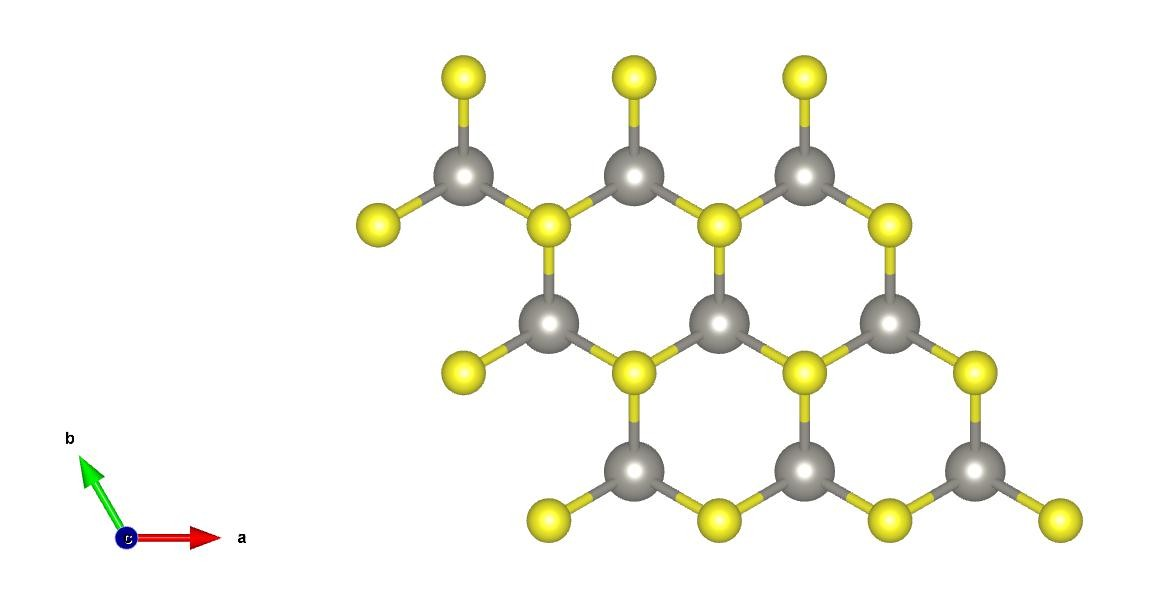
\includegraphics[width=1.0\textwidth]{img/TMDs_structure.jpg} 
\caption{TMDs 晶格結構俯視圖。灰色球體為 $\text{W}$，黃色球體為 $\text{S}$。} 
\label{fig:tmds_structure_a} 
\end{figure} 

\begin{figure}[H] 
\centering 
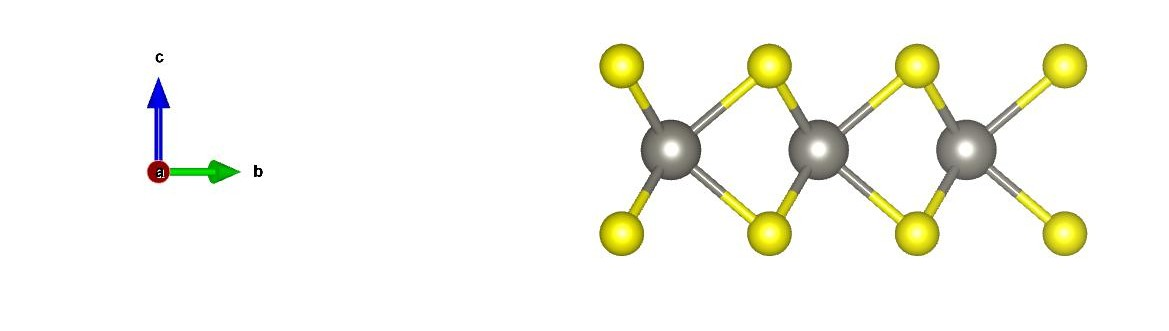
\includegraphics[width=1.0\textwidth]{img/TMDs_structure_2.jpg} 
\caption{TMDs 晶格結構側視圖。灰色球體為 $\text{W}$，黃色球體為 $\text{S}$。} 
\label{fig:tmds_structure_b} 
\end{figure}

\subsubsection*{能帶結構、自旋軌道耦合與激子物理}

在能帶結構方面，過渡金屬原子 (尤其是 W 基材料) 的強自旋軌道耦合 (Spin-Orbit Coupling, SOC) 在 $K$ 點的價帶頂造成顯著的自旋分裂，形成能量不同的上、下兩個自旋子帶。此分裂量在 W 基材料 (WS$_2$、WSe$_2$) 中高達 400–460 meV，在 Mo 基材料 (MoS$_2$、MoSe$_2$) 中約為 140–160 meV。由於時間反演對稱性的限制，$K$ 與 $K'$ 谷的自旋分裂方向恰好相反，形成自旋–谷鎖定效應 (Spin-Valley Locking)：在 $K$ 谷，自旋向上的電子佔據較高的價帶子帶；在 $K'$ 谷，自旋向下的電子佔據對應位置 \cite{xiao2012coupled}。


\begin{figure}[H] 
\centering 
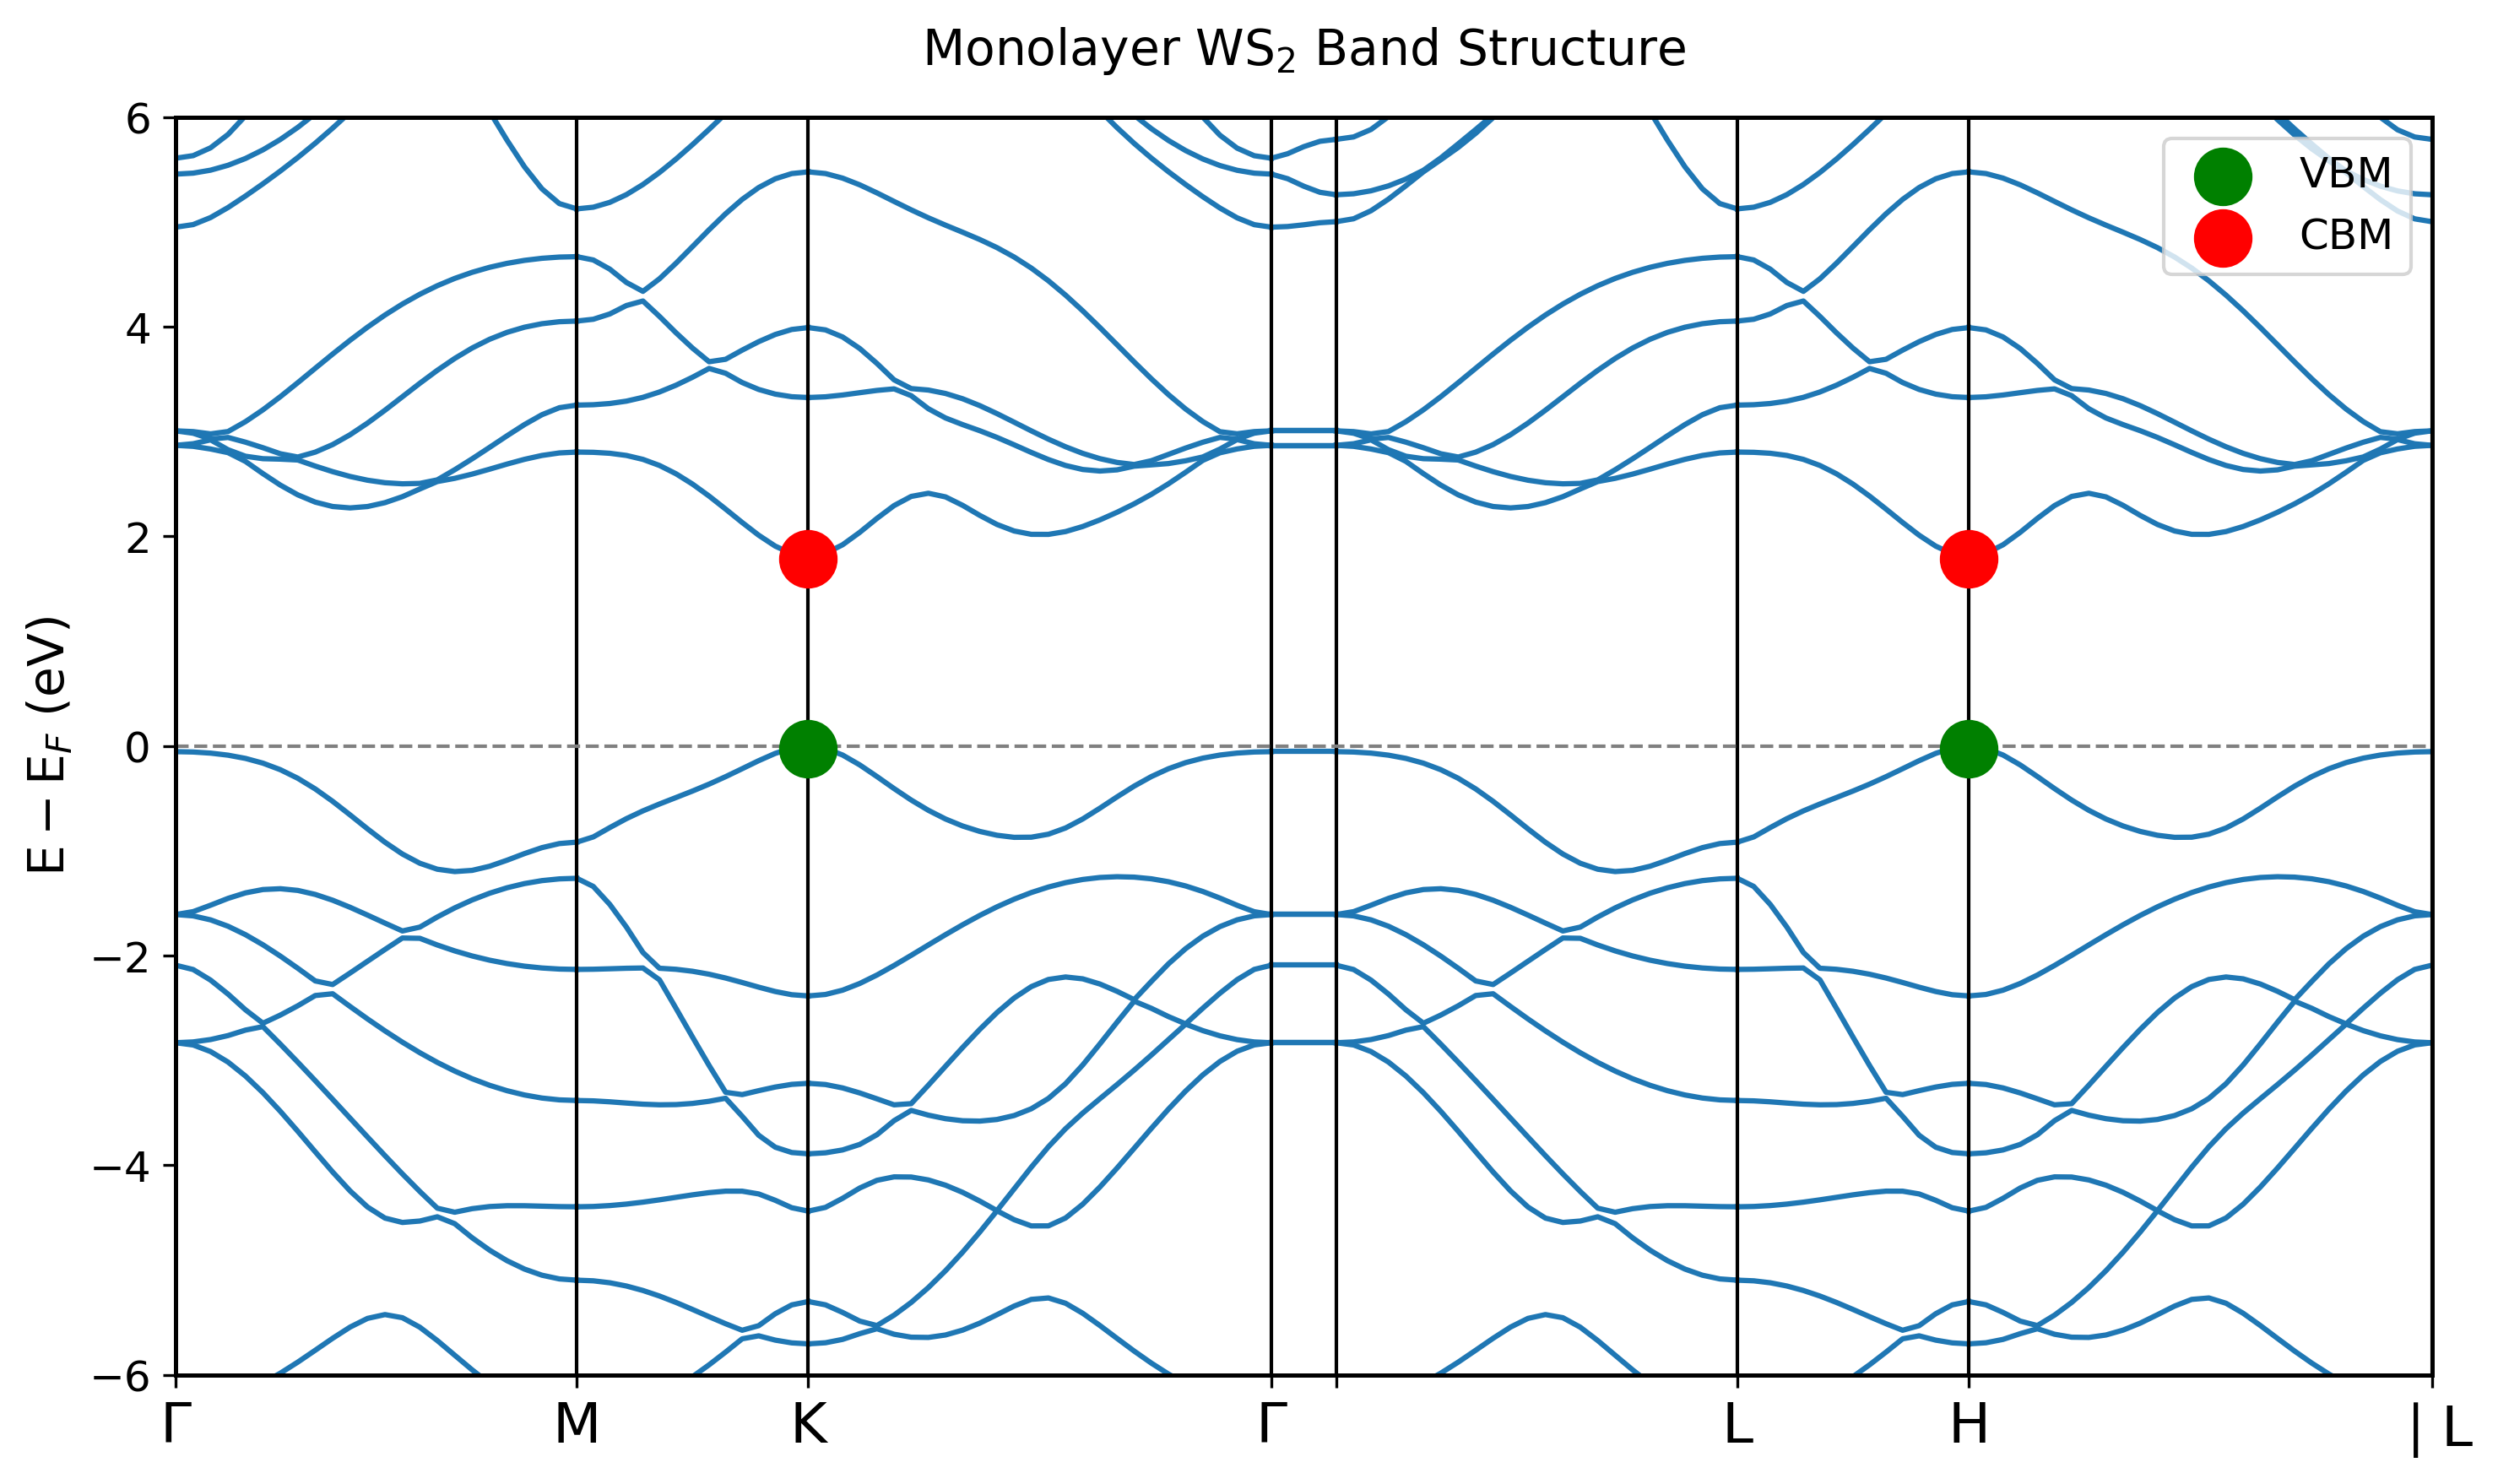
\includegraphics[width=1.0\textwidth]{img/WS2_8points_markers.png} 
\caption{單層 $\text{WS}_2$ 能帶結構圖。$K$ 與 $K'$ ($H$) 谷處的垂直線代表直接能隙位置。綠點為價帶頂 (VBM)，紅點為導帶底 (CBM)，兩者的能量差即為形成 A 激子所需的最小能量。} 
\label{fig:tmds_structure_c} 
\end{figure}

在此能帶結構之上，光學激發所產生的電子-電洞對因強烈的庫倫吸引力而束縛在一起，形成激子 (Exciton) –– 一種由電子與電洞組成的準粒子。相較於三維塊材半導體，二維材料中的庫倫交互作用因介電屏蔽大幅降低而顯著增強，使激子束縛能高達 0.3–0.5 eV，遠大於室溫熱能 ($k_BT \approx 26\text{ meV}$)，確保激子在室溫下依然穩定存在，成為 TMDs 光學響應的主體 \cite{wang2018colloquium}。

依據躍遷所涉及的價帶子帶，可定義兩類激子。A 激子 (A Exciton) 由導帶底至較高自旋子帶 (較靠近費米能的 VB 上子帶) 的躍遷所形成，發光能量較低；B 激子 (B Exciton) 則由導帶底至較低自旋子帶 (VB 下子帶) 的躍遷所形成，兩者發光能量之差即為自旋軌道分裂量 $\Delta_{\text{SOC}}$。在本論文後續的文獻回顧與模擬討論中，所涉及的谷選擇性發光訊號均以 A 激子躍遷為主體。

\subsubsection*{谷選擇定則的量子力學推導}

谷選擇定則的物理根源，可從電偶極光學矩陣元素的對稱性出發進行嚴格推導。在 $D_{3h}$ 點群的約束下，$K$ 與 $K'$ 谷的導帶底 Bloch 態主要由過渡金屬原子的 $d_{z^2}$ 軌道貢獻 (磁量子數 $m = 0$)；而 $K$ 谷與 $K'$ 谷的價帶頂 Bloch 態分別由 $d_{x^2-y^2}$ 與 $d_{xy}$ 軌道組合為 $d_{\pm 2} \equiv  (d_{x^2-y^2} \pm id_{xy})/\sqrt{2}$，等效磁量子數為 $m = \pm 2$，其中正負號分別對應谷指標 $\tau = \pm 1$ ($K$ 谷與 $K'$ 谷)。
光學躍遷的電偶極矩陣元素可以表示為：
\begin{align}
\mathbf{P}_\tau = \langle u_{c,\tau\mathbf{K}} | \hat{\mathbf{p}} | u_{v,\tau\mathbf{K}} \rangle
\end{align}
定義對應左右旋圓偏振光的動量算符 $\hat{p}_\pm = \hat{p}_x \pm i\hat{p}_y$ (分別對應光子角動量 $\pm\hbar$)。由角動量守恆，利用 $D_{3h}$ 不可約表示的選擇定則，可嚴格驗證：
\begin{align}
|\langle u_{c,\mathbf{K}} | \hat{p}_+ | u_{v,\mathbf{K}} \rangle|^2 &\neq 0, \quad |\langle u_{c,\mathbf{K}} | \hat{p}_- | u_{v,\mathbf{K}} \rangle|^2 = 0 \\
|\langle u_{c,\mathbf{K}'} | \hat{p}_+ | u_{v,\mathbf{K}'} \rangle|^2 &= 0, \quad |\langle u_{c,\mathbf{K}'} | \hat{p}_- | u_{v,\mathbf{K}'} \rangle|^2 \neq 0
\end{align}
此嚴格的選擇定則表明：本研究設定下，$\text{K}$ 谷由左旋圓偏振光 ($\text{LCP}, \sigma^-$) 選擇性激發，而 $\text{K}'$ 谷則由右旋圓偏振光 ($\text{RCP}, \sigma^+$) 選擇性激發，展現了光子自旋角動量 (SAM) 與電子谷自由度之間的鎖定關係 \cite{xiao2012coupled}。

在實驗操作上，透過給定螺旋性的圓偏振光對單層 TMDs 進行光學激發，可選擇性地在單一谷中激發電子-電洞對，打破兩谷間的載子平衡，實現動態的谷極化。當這些極化的谷激子發生輻射復合時，其光致發光會繼承激發光的偏振特性，$K$ 谷與 $K'$ 谷的激子發射分別產生高純度的 $\sigma^-$ 與 $\sigma^+$ 圓偏振光。

谷極化發射的純度通常以圓偏振度 (degree of circular polarization, $Pc$) 來量化，定義為左右旋偏振發光強度的差值與總和之比：
\begin{align}
Pc = \frac{I (\sigma^+) - I (\sigma^-)}{I (\sigma^+) + I (\sigma^-)}
\end{align}
由於光子的圓偏振特性在物理本質上即對應於光子的 SAM，單層 TMDs 的谷極化輻射使其成為極具潛力的單光子源與操控光子 SAM 的理想載體 \cite{gong2018nanoscale}。然而，為了進一步提升光學資訊的乘載與處理能力，如何將此固有的谷自由度 (SAM) 進一步轉換為光子的 OAM，成為近代自旋光子學的研究核心。

在超穎表面與全介電質谷光子晶體技術的發展下，透過特殊設計的微奈米結構，已被證實能夠調控並展現具備谷對比特性的 OAM，進而實現谷手性的單向激發 \cite{chen2017valley}。這為晶片整合的量子資訊處理與多維度光學調控提供了全新且關鍵的解決方案。

\subsection{Spin-Orbit Interaction and SAM-to-OAM Conversion}

光子的自旋軌道交互作用  (Spin-Orbit Interaction, SOI) 描述光子的 SAM  (偏振狀態) 與空間 OAM  (波前幾何結構) 之間的相互耦合機制。在不同的光學系統中，SOI 可透過不同的幾何機制被引發：在強聚焦光學系統中，波前的急劇彎曲引發自發性的 SAM 到 OAM 轉換；而在平面奈米光子學中，空間非均勻的幾何相位調控則提供了晶片整合的 SOI 實現路徑。以下分別闡述這兩種機制。

\subsubsection*{強聚焦系統中的自旋軌道交互作用}

當光學系統進入非近軸範疇，SAM 與 OAM 將不再獨立。在強聚焦系統中，光線會以極大的角度向中心匯聚，使得波前發生劇烈彎曲，並在焦點附近形成極具空間不均勻性的橫向電場分佈。此時，其橫向空間梯度 ($\partial E_x/\partial x$ 與 $\partial E_y/\partial y$) 將會大幅增加，為了滿足馬克士威方程式中的高斯定律：
\begin{align}
\nabla \cdot \mathbf{E} = \frac{\partial E_x}{\partial x} + \frac{\partial E_y}{\partial y} + \frac{\partial E_z}{\partial z} = 0
\end{align}
系統必然會產生顯著的縱向電場分量 $E_z$，其振幅大小與橫向分量 $E_x, E_y$ 相當，在數學計算與物理效應上皆不可忽略。這種由幾何邊界與波前結構驅動的場分量耦合轉換，便是引發光學自旋軌道交互作用的核心機制。

為了具體量化此物理現象，以攜帶 SAM  ($s = \pm 1$) 的圓偏振高斯光束經過高數值孔徑透鏡強聚焦為例。當入射光為左旋圓偏振 (LCP, $s = +1$) 時，其入射電場可表示為：
\begin{align}
\mathbf{E}_{in} = \mathbf{E}_{0}  (r,z)  (\hat{x} + is\hat{y})e^{ikz}
\end{align}
若將公式轉換至柱座標系，則可展開為：
\begin{align}
\mathbf{E}_{\text{in}} \propto  (\hat{x} + is\hat{y}) =  (\cos\phi \hat{\rho} - \sin\phi \hat{\phi}) + is (\sin\phi \hat{\rho} + \cos\phi \hat{\phi})
\end{align}
當光線經透鏡聚焦傾斜 $\theta$ 時，由於方位角分量 ($\hat{\phi}$ 項) 始終與 $z$ 軸垂直，只有徑向分量 ($\hat{\rho}$ 項) 會投影到 $z$ 軸。單獨提取 $\hat{\rho}$ 前面的係數，其幾何投影關係為：
\begin{align}
\text{Projection to } z \propto \cos\phi + is\sin\phi = e^{is\phi}
\end{align}
在 Richards-Wolf 高 NA 聚焦理論中，焦點總電場是透過對透鏡孔徑面上的平面波進行二維角譜積分得到。計算縱向電場分量 $E_z$ 的孔徑面方位角環向積分為：
\begin{align}
E_z \propto \int_0^{2\pi} e^{is\phi_p} e^{ik\rho\cos (\phi_p - \phi)} d\phi_p = e^{is\phi} \int_0^{2\pi} e^{is\alpha} e^{ik\rho\cos\alpha} d\alpha
\end{align}
方位角相位 $e^{is\phi}$ 被提到積分符號外面，右側積分項正比於一階第一類貝索函數 $J_1 (k\rho\sin\theta)$。因此，焦平面 ($z=0$) 附近的縱向電場分量可嚴格推導為：
\begin{align}
E_{z} (\rho, \phi, z) = -iAe^{is\phi}I_{1} (\rho,z), \quad I_1 (\rho, z) = \int_0^\alpha \cos^{1/2}\theta \sin^2\theta P (\theta) J_1 (k\rho\sin\theta) e^{ikz\cos\theta} d\theta
\end{align}
其中 $A$ 為振幅常數，$P (\theta)$ 為切趾函數，$\alpha$ 為最大聚焦半角。$E_z$ 中自發性地衍生出拓撲荷 $\ell = s = +1$ 的螺旋相位因子 $e^{is\phi}$，即原本純粹由偏振狀態決定的 SAM，在強聚焦的幾何邊界約束下，部分能量轉換成帶有螺旋波前的 OAM，闡明了強聚焦系統中 SAM 到 OAM 轉換的物理機制。

\subsubsection*{幾何相位 (Pancharatnam–Berry Phase)與平面奈米光子學中的 SOI}

上述強聚焦 Richards–Wolf 推導揭示，SAM 到 OAM 的轉換本質上源自於空間相位梯度與偏振態的幾何耦合。在平面奈米光子學元件的設計框架中，實現此類 SOI 轉換並不依賴大數值孔徑透鏡系統，而是透過另一種更適合晶片整合的機制––幾何 (Pancharatnam–Berry)相位––來完成。

幾何相位的物理根源最早由 Pancharatnam 於 1956 年在光學干涉的情境中提出 \cite{pancharatnam1956generalized}，後由 Berry 於 1984 年推廣為量子力學的普遍原理 \cite{berry1984quantal}：當一個量子態在參數空間中沿閉合路徑絕熱演化回到初態時，除積累動力學相位外，還會額外獲得一個僅由演化路徑幾何形狀決定的相位。在光學偏振的情境中，偏振態可以用龐加萊球 (Poincaré Sphere)上的一點表示：北極對應右旋圓偏振 ($\sigma^+$)，南極對應左旋圓偏振 ($\sigma^-$)，赤道上各點對應不同方位角的線偏振態。當偏振態在 Poincaré 球面上沿一閉合路徑演化時，所積累的 Pancharatnam–Berry 相位 (PB 相位) 等於該路徑在球面上所圍固體角 $\Omega_\text{solid}$ 之半：
\begin{align}
\Phi_{\text{PB}} = \frac{\Omega_\text{solid}}{2}
\end{align}
對於一個局部雙折射奈米天線，當其快軸旋轉角度 $\theta$ 時，通過後的交叉極化分量在 Poincaré 球上的演化路徑從 $\sigma^+$ 出發，經由赤道上旋轉 $2\theta$ 的線偏振中間態到達 $\sigma^-$，整個閉合路徑所圍固體角為 $4\theta$，因此 PB 相位為：
\begin{align}
\Phi_{\text{PB}} = \frac{4\theta}{2} = 2\theta
\end{align}
此結果表明，PB 相位的符號與大小完全由天線的空間旋轉角度 $\theta$ 決定，而與波長無關，賦予幾何相位超穎表面優越的寬頻特性。

基於上述 PB 相位的物理根源，考慮一局部雙折射奈米結構 (如超穎表面的天線單元)，假設其快軸相對於參考軸的局部方位角為 $\theta (\phi)$，其中 $\phi$ 為方位角。當一圓偏振光 ($\sigma_z = \pm 1$) 入射該結構時，穿透或反射的光場除了包含保持原偏振的共極化分量外，還會產生一個手性相反的交叉極化分量。該交叉極化分量會額外獲得一個與結構空間方位直接相關的幾何相位移：
\begin{align}
\Omega = \mp 2\theta (\phi)
\end{align}
若進一步將奈米結構的空間方位設計為隨方位角呈線性變化，即滿足關係式 $\theta (\phi) = q\phi$ (其中 $q$ 為半整數或整數)，則入射的圓偏振光在通過該結構後，其交叉極化分量所附加的幾何相位將演變為 $\exp (\mp i 2q\phi)$。根據 \ref{ssec:oam of light} 對螺旋相位的定義，此方位角相關的相位分佈正對應於拓撲荷為 $\ell = \mp 2q$ 的 OAM 模態。

幾何相位超穎表面為實現 SAM 到 OAM 轉換提供了最具代表性的有效平台之一。然而更廣義而言，光子的 SOI 可透過在空間中非均勻分佈的光學響應進行任意調控。藉由打破傳統單元結構旋轉的局部幾何相位限制，可在更廣義的二維非均勻介質中，自由操控空間相位梯度，進而實現具備客製化 OAM 狀態的任意結構光場。這為利用新型非直覺光學結構調控波前、產生高純度 OAM 模態奠定了理論基礎。

\subsection{Inverse Design and Topology Optimization}

在奈米光學元件的傳統設計方法中，通常採用正向設計，即依賴物理直覺或既有的經驗幾何圖形 (如圓柱、矩形天線) 進行有限的參數掃描。然而，這種方法強烈受限於人類的幾何直覺，且僅能調控極少數的自由度，難以應對非直覺、多功能或極端非對稱的高難度光場調控需求。

為了突破傳統設計的瓶頸，反向設計方法應運而生。反向設計將光學元件設計轉化為一個嚴謹的數學最佳化問題：首先定義一個具體描述目標性能的目標函數 (Figure of Merit, FOM)，再從目標結果出發，反向尋找最優的空間介電常數分佈。

在面對高維度設計空間時，結合伴隨變量法的拓樸最佳化展現出極大的數值優勢。伴隨變量法僅需進行兩次全波電磁模擬 (正向模擬與反向伴隨模擬)，即可高效計算出目標函數對於成千上萬個空間網格的精確梯度。藉由梯度下降等最佳化演算法，拓樸最佳化能在奈米尺度下自由調整物質的幾何邊界與拓撲結構，從而在龐大的參數空間中自動演化出超越傳統直覺的高性能光學結構，為實現理想光學結構提供了強大的核心數值方法支撐。

\section{State of Related Research}

\subsection{Metasurface-based OAM Generation}

模態純度已成為最重要的指標之一，用於評估 OAM 產生器的性能。

早期的 OAM 超穎表面多採用電漿子金屬奈米天線陣列，例如 Karimi 等人於2014年利用空間漸變的超薄 L 型金奈米結構，在可見光波段實現了基於幾何相位的 OAM 渦旋產生器 \cite{karimi2014generating}。然而，純粹依賴離散奈米天線的相位調控易產生相位雜訊，激發的高階徑向模態常使出射光束產生多重同心圓環的非理想光場分佈 \cite{karimi2014generating}。為了解決上述缺陷並提升模態純度，Guo 等人提出將幾何相位與電漿子延遲相位結合於連續形狀的超穎表面中，成功將拓樸荷 $\ell = 2$ 的光學渦旋純度從離散結構的 $64\%$ 提升至 $90\%$ 以上 \cite{guo2016merging}，特別強調了相位分佈的幾何連續性對於抑制模態串擾和提高 OAM 純度方面的重要性。

為突破電漿子材料的損耗限制，近年的研究主流轉向低損耗的介電質平面光學與全介電質超穎表面。針對傳統 OAM 光環尺寸隨拓撲荷增加而發散的應用瓶頸，Liu 等人於2017年提出利用超薄的石英玻璃平面相位元件，實驗上成功產生了光環尺寸獨立於拓撲荷的完美渦旋光束，大幅縮小了傳統光學系統的體積 \cite{liu2017generation}。這些高純度的腔外調控技術進一步促成了光電系統的發展，例如 Bi 等人於2018年與 Tan 等人於2019年分別在毫米波段與自由空間光通訊中實現了寬頻與多工傳輸 \cite{bi2018metasurface, tan2019free}。另一方面，如何在複雜的多工影像重建中保持 OAM 的空間相位特徵並抑制像素間的模態串擾，Ren 等人於2019年提出了空間頻率採樣與相位補償技術 \cite{ren2019metasurface}，該研究揭示了遠場干涉對 OAM 螺旋波前的破壞機制，並藉由傅立葉空間離散採樣與基態濾波技術，成功抑制了重建像素間的螺旋波前干涉與模態串擾，為高容量空間光學多工系統奠定基礎。

儘管上述腔外系統取得諸多進展，其純度依然受限於元件加工精度與傳播繞射。為突破此純度極限，Sroor 等人於 2020 年首創將二氧化鈦全介電質超穎表面整合至雷射共振腔內\cite{sroor2020high}。該研究證實，雷射腔內的繞射、共振與增益輔助濾波機制能自然過濾掉不需要的徑向散射模態，即使在 $\ell=100$ 的極高階 OAM 狀態下，依然能有效抑制高階徑向模態，將 $p=0$ 的目標模態純度維持在近 $90\%$ 。 在此技術發展的基礎上，為了進一步提升設計自由度，Zhou 等人於 2021 年利用二氧化鈦全介電質幾何超穎表面，成功生成了光環半徑獨立於拓撲荷變化的完美渦旋光束，展示了能在單一元件上，同時獨立調控光束尺寸與橢圓率等多維度特徵的能力 \cite{zhou2021generation}。

儘管現有的 OAM 超穎表面已展現卓越性能，但現行元件主要仍依賴基於單元結構的正向設計方法，即透過排列特定形狀的奈米天線來實現相位調控。預先定義的幾何模板嚴格限制了此類設計的自由度。雖然高純度的 OAM 光束已在上述文獻中被個別驗證，但其元件表現依然強烈依賴這些特定的原子幾何與相位工程策略，難以在多目標光場調控中達到全局最佳化。

\begin{table}[h]
\centering
\caption{超穎表面 OAM 產生技術發展年表}
\label{tab:timeline_oam}
\small
\begin{tabular}{c p{11cm}}
\toprule
\textbf{年份} & \textbf{文獻重點} \\
\midrule
2014 & 以漸變 L 型金奈米結構陣列實現幾何相位 OAM 渦旋產生器，驗證電漿子超穎表面生成渦旋光 \cite{karimi2014generating} \\
2016 & 幾何相位與延遲相位結合，連續形超穎表面將 OAM 模態純度從 64\% 提升至 90\% 以上 \cite{guo2016merging} \\
2017 & 石英玻璃平面相位元件產生完美渦旋光束，光環尺寸獨立於拓撲荷大小 \cite{liu2017generation} \\
2018 & 超穎表面實現毫米波 OAM 多工寬頻傳輸 \cite{bi2018metasurface} \\
2019 & 超穎表面實現自由空間光通訊 OAM 多工傳輸 \cite{tan2019free} \\
2019 & 空間頻率採樣與相位補償技術抑制 OAM 多工重建中的螺旋波前干涉 \cite{ren2019metasurface} \\
2020 & TiO$_2$ 超穎表面整合至雷射共振腔，$\ell=100$ 高階 OAM 模態純度仍維持近 90\% \cite{sroor2020high} \\
2021 & TiO$_2$ 幾何超穎表面生成完美渦旋光束，在單一元件上獨立調控光束尺寸與橢圓率 \cite{zhou2021generation} \\
\bottomrule
\end{tabular}
\end{table}

\subsection{Valley-controlled Chiral Photonics}

TMDs 因空間反轉對稱性破缺與強 SOC 的協同作用，催生了獨特的自旋能谷鎖定效應 \cite{xiao2012coupled}。圓偏振光可選擇性調控電子的谷自由度，並能透過偏振解析光致發光光譜進行高效的光學初始化與檢測 \cite{mak2012control, zeng2012valley, schaibley2016valleytronics}。

然而，單層 TMDs 中的激子壽命與谷極化壽命通常極短 (僅約數個皮秒)，這極大地限制了谷資訊的邏輯運算與在晶片上的長距離空間傳輸 \cite{schaibley2016valleytronics, gong2018nanoscale}。為了克服此關鍵退相干與損耗瓶頸，學界主要沿著兩條互補的技術路徑展開探索：一是聚焦於利用微奈米光學共振腔的 Purcell 效應提高局域光子態密度，以加速單層 TMDs 的激子自發輻射速率並提升其發光效率 \cite{mak2016photonics, gan2013controlling}；然而，傳統微腔往往缺乏手性選擇性，無法主動維持或操縱激子的谷極化特徵 \cite{mak2016photonics}。另一條更具針對性的路徑，則是利用二維材料固有的谷選擇性圓偏振光學躍遷定則 \cite{xiao2012coupled}，將其與具備光學自旋動量鎖定特性的一維導波結構進行近場耦合，從而建立奈米尺度下的手性能谷光子介面，實現谷極化資訊的定向提取與晶片上傳輸。

其中最具代表性的是Gong 等人於2018年的研究 \cite{gong2018nanoscale}。在具體實作上，該研究將少層 $\text{WS}_2$ 與單根銀奈米線近場耦合。利用表面電漿子極化子波導模態因光學 SOC 所攜帶的本徵橫向光學自旋角動量，達成光學自旋動量鎖定，從而將少層材料中谷選擇性激發的近場圓偏振偶極發光，高效率地轉化為該模態的單向定向傳輸，其定向耦合效率高達 $90 \pm 1\%$。此工作成功建立了奈米尺度下的手性谷-光子介面，也證實了在室溫下進行谷資訊面內傳輸的可行性。

儘管金屬導波結構能藉由電磁場的強局域化實現極高耦合效率，但金屬本徵的高歐姆損耗卻嚴重限制了谷資訊的實際傳輸距離。為了解決此損耗瓶頸，後續研究開始探索TMDs與低損耗的全介電質、高折射率奈米波導或光子晶體波導進行耦合。在這一領域，將二維材料與低損耗、高折射率全介電質微腔整合以調控激子發光的實驗先驅，首推 Gan 等人於 2013 年的研究 ，以及隨後 Wu 等人於 2014 年的研究 \cite{gan2013controlling, Wu2014control}。在這些工作中，學者打破了傳統將發光介質嵌入光子晶體內部的結構限制，首次將單層二維材料轉移至預先製備的 GaP (磷化鎵) 光子晶體微腔表面；這不僅完美避免了蝕刻製程對二維材料激子特性的破壞，更在實驗上觀測到自發輻射速率的有效調控 \cite{gan2013controlling, Wu2014control}。

近年來的研究進一步朝向更小模態體積與超穎表面調控的方向發展。例如，Sortino 等人於 2019 年的研究採用了GaP 奈米天線，與單層及雙層 $\text{WSe}_2​$ 進行近場耦合 \cite{sortino2019enhanced}。該研究利用極小模態體積的低損耗 $\text{GaP}$ 共振腔，在完全避免金屬非輻射與歐姆損耗的同時，實現了高達 $10^4$ 以上的光致發光強度增強，並透過 Purcell 效應使激子輻射衰期縮短至系統偵測極限。這一系列從光子晶體微腔到介電質奈米天線的進展證實了，全介電質 GaP 奈米結構能有效克服金屬的損耗瓶頸，成為高效操控二維激子發光的優異平台。

除了在晶片表面進行面內的定向波導，如何主動調控谷極化發光在自由空間中的三維輻射行為，亦成為另一關鍵課題。透過在 TMDs 表面建構人工設計的全介電質手性超穎表面，學者得以在避免歐姆損耗的前提下實現面外波前調控，進而發展出低損耗的手性超穎表面、谷選擇性全息投影以及攜帶 OAM 的渦旋光束發射。

在面外三維空間調控的實驗中，如何打破系統的面外對稱性以高效提取特定手性的谷極化光子是核心挑戰。為此，Rong 等人於 2020 年的研究取得了突破性進展 \cite{rong2020photonic}。研究使用多晶矽介電質材料以避免金屬損耗，並激發了光子拉希巴 (Rashba) 效應，成功將單層 $\text{WSe}_2$ 的內稟谷自旋轉化為向自由空間特定方向輻射的自旋鎖定窄光束，達成了極高指向性的面外波束成型。

隨著奈米光學與二維材料光電元件的快速演進，研究視野已從傳統的面內定向導波，跨越至如何高效提取並調控自由空間的面外手性輻射。然而，在建構主動式手性光源元件時，研究面臨著根本性的物理挑戰：直接能隙的單層 TMDs 雖具有極高的激子輻射效率與內稟谷自旋選擇性，但其原子級的超薄厚度 (約 $0.7\text{ nm}$) 卻限制了局域電磁場的交互作用與相位調控能力；相反地，雖然多層材料或直接對 TMDs 進行亞波長圖案化的無源器件能提供足夠的幾何相位調控，但多層 TMDs 因轉變為間接能隙，其發光效率呈指數級衰減。因此，將高發光效率的單層 TMD 活性層，與低損耗、高折射率介電質超穎表面進行混合整合，已成為構建二維手性光源與雷射晶片的最佳技術路徑。

在這一技術路徑上，近期的研究取得了里程碑式的進展。例如，Rong 等人於 2023 年的研究將單層 $\text{WS}_2$ 轉移至 $\text{Si}_3\text{N}_4$ Kagome 光子晶體晶格表面，藉由打破空間反轉對稱性激發光子 Rashba 效應，在室溫下成功實現了高相干性的自旋-谷鎖定單層雷射 \cite{rong2023spin}。隨後，Pan 等人於 2025 年的研究則利用矽手性超穎表面激發高活性、強手性近場增強的非局域準連續域束縛態，在室溫下將單層 $\text{MoSe}_2$ 的谷選擇性發光圓偏振極化度提升至新高 \cite{pan2025room}。

儘管這些基於高品質因子腔體的混合元件在提升手性提取效率與激子輻射速率上表現優異，但目前的設計仍存在顯著的技術瓶頸。現有元件多依賴於週期性、高度對稱的常規晶格幾何 (如 Kagome 晶格或切角正方形陣列) ，這使得其遠場波前調控能力通常被局限於簡單的定向偏折窄光束或多對稱輻射點。在無需外部偏振濾光片的前提下，如何直接對單層 TMD 激子的自發輻射進行高自由度的複雜波前塑形 (例如直接產生攜帶 OAM 、高模態純度的渦旋光束或 LG 模態) ，並同時維持極高的谷極化選擇性，依然是當前自旋-谷光電子晶片面臨的核心瓶頸。

\begin{table}[h]
\centering
\caption{谷手性光子學研究發展年表}
\label{tab:timeline_valley}
\small
\begin{tabular}{c p{11cm}}
\toprule
\textbf{年份} & \textbf{文獻重點} \\
\midrule
2012 & 理論預測單層 TMDs 因反轉對稱破缺形成自旋能谷鎖定，建立谷選擇性光學躍遷定則 \cite{xiao2012coupled} \\
2012 & 實驗驗證 MoS$_2$ 谷極化光學初始化，以圓偏振光選擇性激發單一能谷 \cite{mak2012control} \\
2012 & 確認 WSe$_2$ 谷選擇性圓偏振光致發光，奠定谷電子學實驗基礎 \cite{zeng2012valley} \\
2013 & 首次將單層二維材料轉移至 GaP 光子晶體微腔表面，觀測自發輻射速率調控 \cite{gan2013controlling} \\
2014 & GaP 光子晶體微腔調控單層 TMD 激子自發輻射速率，驗證介電質腔與二維材料整合 \cite{Wu2014control} \\
2016 & 系統回顧谷電子學進展，指出皮秒激子壽命限制谷資訊在晶片上的長距離傳輸 \cite{schaibley2016valleytronics} \\
2018 & WS$_2$ 與銀奈米線近場耦合，谷選擇性定向耦合效率達 $90\pm1$\% \cite{gong2018nanoscale} \\
2019 & GaP 奈米天線與 WSe$_2$ 近場耦合，PL 增強 $10^4$ 倍並透過 Purcell 效應縮短輻射衰期 \cite{sortino2019enhanced} \\
2020 & 多晶矽超穎表面激發光子 Rashba 效應，將 WSe$_2$ 谷自旋轉化為定向自旋鎖定窄光束 \cite{rong2020photonic} \\
2023 & 單層 WS$_2$ 結合 Si$_3$N$_4$ Kagome 光子晶體，室溫實現自旋-谷鎖定相干雷射 \cite{rong2023spin} \\
2025 & 矽手性超穎表面激發準 BIC 強手性近場，室溫大幅提升 MoSe$_2$ 谷選擇性圓偏振度 \cite{pan2025room} \\
\bottomrule
\end{tabular}
\end{table}

\subsection{Existing Valley-to-OAM Conversion Platforms}

關於現存的能谷與 OAM 轉換技術，近期的研究主要依賴能谷軌道耦合效應或特定的光子共振態來實現。

部分學者利用應力陷阱在單層半導體中捕捉層內激子，藉由電子-電洞庫倫交換作用所介導的激子質心動量與能谷自由度的本徵耦合，在奈米尺度下實現了光子 SAM 與 OAM 鎖定的單光子發射 \cite{zhang2023single}。此外，亦有研究將非中心對稱的 TMDs 圖案化為光子晶體超穎表面，使其與連續體束縛態 (Bound States in the Continuum, BIC) 發生強耦合形成激子極化子\cite{li2023valley}。在此物理圖像中，BIC 的拓撲荷 $q$ 被定義為動量空間中偏振主軸角度 $\phi(k)$ 沿閉合路徑 $C$ 的積分，其關係式可表示為 $q=\frac{1}{2\pi}\oint_{C}dk\cdot\nabla_{k}\phi(k)$。此拓撲特性賦予了遠場輻射的偏振渦旋結構，藉由自旋-谷鎖定選擇定則，成功將 TMDs 的能谷自由度與光子 OAM 的拓撲荷直接連結 \cite{li2023valley}。此種由能谷物理主導的手性調控，近年亦被成功推廣至人工拓撲光子平台。同時，結合克庫勒調變的自製狄拉克渦旋微腔，亦被證實能透過能谷間耦合與自旋能谷鎖定的協同機制，自發輻射出具備高度自旋軌道角動量鎖定 (Spin-orbit angular momentum locking) 的特定 OAM 渦旋光束 \cite{li2026unveiling}。

儘管上述研究成功實現了能谷資訊與光波 OAM 的結合，這些技術路線仍面臨純度受限與調控彈性不足的雙重挑戰。應力陷阱方法雖能產生具備 OAM 的單光子，但應力分佈的隨機性與周遭環境干擾容易導致出射光純度下降；而結合 BIC 或克庫勒調變的超穎表面，其生成的 OAM 階數高度依賴於固定的晶格對稱性 (如四重旋轉對稱)，難以在單一元件上進行動態且彈性的高階模態切換。更為關鍵的是，目前學界仍缺乏一個能直接將谷極化高純度轉換為特定 LG 模態的直接轉換平台。

因此，如何突破既有平台受限於特定共振機制與晶格對稱性的限制，建立具有更高設計自由度的 Valley-to-OAM 轉換架構，已成為目前的重要研究方向。

\begin{table}[h]
\centering
\caption{現有能谷–OAM 轉換平台研究年表}
\label{tab:timeline_v2oam}
\small
\begin{tabular}{c p{11cm}}
\toprule
\textbf{年份} & \textbf{文獻重點} \\
\midrule
2023 & 應力陷阱捕捉層內激子，庫倫交換作用介導 SAM–OAM 鎖定的單光子發射 \cite{zhang2023single} \\
2023 & TMDs 光子晶體超穎表面與 BIC 強耦合，谷自由度與光子 OAM 拓撲荷直接連結 \cite{li2023valley} \\
2026 & 克庫勒調變狄拉克渦旋微腔透過自旋能谷鎖定機制，自發輻射高純度 OAM 渦旋光束 \cite{li2026unveiling} \\
\bottomrule
\end{tabular}
\end{table}

\subsection{Inverse-designed Nanophotonic Devices}

傳統的奈米光子元件設計高度依賴物理直覺與有限的幾何參數掃描，面臨結構複雜化帶來的瓶頸。為突破限制，自動化尋找光學結構的反向設計近年成為奈米光子領域的核心技術 \cite{jensen2011topology, molesky2018inverse}。其中，拓撲最佳化賦予設計空間最大的自由度；與傳統以單元結構為基礎的正向設計不同，拓撲最佳化不需預先假設結構形狀，而是在連續設計空間中直接搜尋最佳介電質分布，從而探索出非直觀的結構 \cite{jensen2011topology}。因此，這種方法特別適合需要同時最佳化振幅、相位、偏振與模態純度等多重目標的複雜波前設計。為在龐大自由度中高效收斂，伴隨變量法至關重要，其僅需前向與伴隨兩次電磁場模擬即可高效計算出目標函數對所有幾何參數的梯度，極大幅降低了計算成本，使複雜光子元件的自動化設計成為可能。

在超穎表面的研究中，反向設計展現了強大的多功能整合與光場調控能力。近期成果已廣泛涵蓋高效率非對稱光束偏轉 \cite{li2022empowering}、大數值孔徑消色差超透鏡聚焦 \cite{choi2025roll}、全斯托克斯偏振成像偵測 \cite{wang2024non} 及多維多通道複用全像顯示 \cite{yin2024multi}。這些自由曲面元件透過拓撲最佳化達到了傳統幾何結構無法企及的傳輸效率與功能密度，證明了反向設計在操縱複雜光場上的成熟度與優勢。

然而，綜觀現有的反向設計超穎表面研究，其核心機制主要聚焦於空間中光波之振幅、相位與偏振的基本調控 \cite{molesky2018inverse, li2022empowering}。

相較之下，將反向設計應用於二維材料的谷發射器調控仍處於起步階段。現有 TMDs 的谷發射調控多依賴傳統物理直覺設計的電漿子或奈米線結構 \cite{mak2012control, deng2021plasmonic}。雖然已有研究將反向設計與單層 TMDs 結合以進行腔耦合或暗激子偵測 \cite{gelly2023inverse}，但針對特定谷手性的高自由度發射調控仍極為稀缺。更具挑戰性的是，目前極少有研究探討如何將特定谷自由度的手性圓偏振發光，直接轉換為攜帶 OAM 的 LG 光束。

儘管矽晶片已能實現高效的反向設計 OAM 發射器 \cite{white2023inverse}，目前還未有同時進行動量匹配、手性選擇與空間模態變換的谷選擇性反向設計發射器。此一研究缺口正是本文所欲探討與解決的核心課題。

\begin{table}[h]
\centering
\caption{反向設計奈米光子元件研究發展年表}
\label{tab:timeline_inverse}
\small
\begin{tabular}{c p{11cm}}
\toprule
\textbf{年份} & \textbf{文獻重點} \\
\midrule
2011 & 提出拓撲最佳化框架，以梯度法在奈米光子設計空間中自動搜尋最佳介電分布 \cite{jensen2011topology} \\
2018 & 系統性回顧奈米光子逆設計理論，建立反向設計最佳化通用框架 \cite{molesky2018inverse} \\
2022 & 拓撲最佳化超穎表面實現高效非對稱光束偏轉，超越傳統正向設計上限 \cite{li2022empowering} \\
2023 & 反向設計結合單層 TMD 進行腔耦合優化與暗激子偵測 \cite{gelly2023inverse} \\
2023 & 反向設計矽基 OAM 發射器，驗證逆設計於主動式 OAM 元件的可行性 \cite{white2023inverse} \\
2024 & 反向設計超穎表面實現全斯托克斯偏振成像偵測 \cite{wang2024non} \\
2024 & 拓撲最佳化超穎表面實現多維多通道複用全像顯示 \cite{yin2024multi} \\
2025 & 反向設計實現大數值孔徑消色差超透鏡聚焦 \cite{choi2025roll} \\
\bottomrule
\end{tabular}
\end{table}

\section{Research Gap and Thesis Motivation}

綜觀上述研究，目前基於超穎表面的 OAM 產生技術已具備成熟的遠場波前調控能力 \cite{liu2017generation, sroor2020high}，而谷電子手性光子學亦已能有效操控單層 TMDs 的谷極化發光 \cite{xiao2012coupled, gong2018nanoscale}。然而，如何在同一奈米光子平台中，同時實現谷選擇性與高自由度結構光控制之自由空間發射，仍然是一項尚未解決的重要課題。

根據目前的研究進展，現存技術主要面臨兩項核心研究缺口。首先，現有的能谷與結構光結合平台受限於特定物理機制與幾何對稱性。現行研究高度依賴應力陷阱 \cite{zhang2023single}、BIC \cite{li2023valley} 或克庫勒調變的狄拉克渦旋微腔 \cite{li2026unveiling}，其生成的 OAM 階數高度受限於固定的晶格幾何，難以進行彈性調控，導致目前仍缺乏能進行高自由度結構光控制的通用平台。其次，現有的反向設計技術在谷光子學領域的應用仍相當受限。雖然反向設計與拓撲最佳化技術已在無源超穎表面上展現強大的光場調控成熟度 \cite{li2022empowering, yin2024multi}，但其核心機制主要聚焦於外部入射光波的調控 \cite{molesky2018inverse}，針對二維材料主動發射調控的研究仍處於起步階段 \cite{gelly2023inverse}。因此，目前仍缺乏專為谷選擇性反向設計發射器設計的反向設計平台。尤其是在同一元件中，同時兼顧動量匹配、谷選擇性與遠場空間模態轉換的設計架構仍相當有限 \cite{white2023inverse}。

為解決上述研究缺口，本研究提出一套以低損耗、高折射率全介電質平台為基礎之谷選擇性反向設計發射器，並以 $\text{GaP}$ 作為實作材料，結合時域有限差分法 (Finite-Difference Time-Domain, FDTD) 與伴隨變量法進行全局反向設計 \cite{jensen2011topology}。本研究以 LG 光束作為代表性的結構光設計目標，透過對單層 $\text{WS}_2$ 激子發光進行反向設計，以打破傳統週期性晶格的對稱性限制。本研究建立一種可直接將單層 $\text{WS}_2$ 激子發光轉換為高純度 LG 光束之設計架構，在無需外部偏振濾光片的條件下，同時保留並區分二維材料內稟的谷極化資訊，並提供一種兼具谷選擇性與複雜波前控制能力之主動式奈米光子元件設計策略。